\documentclass[a4paper]{article}
\usepackage[frenchb]{babel}
\usepackage[utf8]{inputenc}
\usepackage{Sweave}
\usepackage{url}
\usepackage{graphicx}
\usepackage{pdfpages}
\usepackage{geometry}
\geometry{hmargin=2.5cm,vmargin=1.5cm}

\newlength{\fancyvrbtopsep}
\newlength{\fancyvrbpartopsep}
\makeatletter
\FV@AddToHook{\FV@ListParameterHook}{\topsep=\fancyvrbtopsep\partopsep=\fancyvrbpartopsep}
\makeatother
\setlength{\fancyvrbtopsep}{1pt}
\setlength{\fancyvrbpartopsep}{1pt}
\newcommand{\R}{\textbf{R}}

\title{Correction des Exercices du TD4}
\date{}
\begin{document}
\includepdf{file.pdf}
\Sconcordance{concordance:TP3_M1MAS.tex:TP3_M1MAS.Rnw:%
1 61 1 1 2 1 0 5 1 1 2 1 0 1 1 8 0 1 1 4 0 1 2 15 1 1 2 1 0 5 1 1 2 1 0 %
1 1 7 0 1 1 4 0 1 2 2 1 1 2 1 0 5 1 1 4 3 0 1 2 1 0 1 2 1 0 1 3 1 0 1 2 %
1 0 1 2 1 0 1 2 1 0 1 2 1 0 1 2 10 0 1 2 8 1 1 2 1 0 5 1 1 2 1 0 1 1 11 %
0 1 2 3 1 1 2 1 0 3 1 1 3 1 0 1 1 6 0 1 2 1 0 1 2 1 0 1 2 6 0 1 3 7 1 1 %
2 1 0 4 1 1 2 1 0 1 4 3 0 1 4 3 0 1 2 16 0 1 2 36 0 1 2 24 0 1 2 16 0 1 %
9 7 0 1 3 1 0 1 1 22 0 1 1 4 0 1 2 1 1}

\setkeys{Gin}{width=0.5\textwidth}
\maketitle{}
\paragraph{Objectifs}
\begin{itemize}
 
\item Savoir faire une classification par CAH ou k-means  avec \R.
\end{itemize}
La CAH (classification ascendante hierarchique peut se faire avec la fonction "hclust" de la libraire MASS ou "eclust" de factoextra ou HCPC de la librairie FactoMineR sur les résultats d'une analyse factorielle.). La classification par moyennes mobiles (K-means) peut se faire avec la fonction "eclust" de factoextra.
\section{Exemple} 

Soit la matrice  de données suivante les observations de 2 variables sur $n=4$ indidivus.
$$\displaystyle X=\left(\begin{array}{cc}
2 &12\\
4 & 10\\
5 & 7\\
4 & 5\\
\end{array}\right)
$$
Faisons les classifications CAH et K-means (Moyenne mobiles) avec la distance euclidienne.
\begin{itemize}
\item CAH
\begin{itemize}

\item Matrice des distances

 
\begin{tabular}{|l||r|r|r|}
\hline
			&x1 &x2 &x3\\   
\hline
\hline   
x2 & $\sqrt 8$ &  & \\    
x3&  $\sqrt{34}$&  $\sqrt{10}$  &\\
x4 & $\sqrt{53}$&  5&  $\sqrt{5}$\\
\hline
\end{tabular}


\begin{Schunk}
\begin{Sinput}
> library("FactoMineR")
> library("factoextra")
> A=matrix(c(2,12,4,10,5,7,4,5),ncol=2, byrow=TRUE)
> X=as.data.frame(A)
> colnames(X)=c("var1", "var2")
> rownames(X)=c("x1", "x2", "x3","x4")
> # Distance euclidienne
> dist <- dist(X, method = "euclidean")
> dist
\end{Sinput}
\begin{Soutput}
         x1       x2       x3
x2 2.828427                  
x3 5.830952 3.162278         
x4 7.280110 5.000000 2.236068
\end{Soutput}
\begin{Sinput}
> fviz_dist(dist, lab_size = 8)
\end{Sinput}
\end{Schunk}
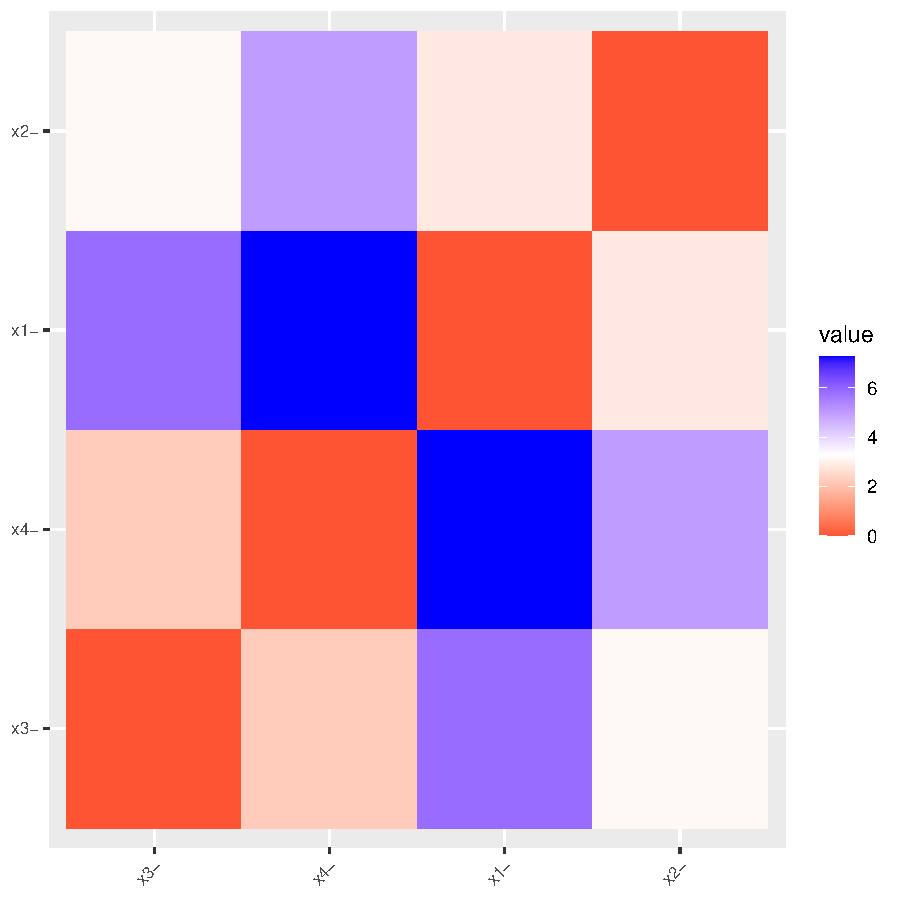
\includegraphics{TP3_M1MAS-001}


\item Etape 1: Les 2 individus les plus proches sont $x_3$ et $x_4$, $d(x_3,x_4)=2.23$ est la plus petite, on les regroupe, le centre du groupe composé de ces 2 individus est $g_{34}=(4.5,6)$ (noeud 5). 
Le saut de ward correspondant est $(1/2)d(x_3,x_4)=1.115$.

On recalcule les distances entre $x_1$ et $x_2$ et $g_{34}$. La matrice des distances est\\
\begin{tabular}{|l||r|r|r|}
\hline
			&x1 &x2 &$g_{34}$\\   
\hline
\hline   
x2 & $\sqrt 8$ &  & \\    
$g_{34}$&  $\sqrt{42.25}$&  $\sqrt{16.25}$  &\\
\hline
\end{tabular}
\item Etape 2:
\begin{Schunk}
\begin{Sinput}
> library("FactoMineR")
> library("factoextra")
> A=matrix(c(2,12,4,10,4.5,6),ncol=2, byrow=TRUE)
> X=as.data.frame(A)
> colnames(X)=c("var1", "var2")
> rownames(X)=c("x1", "x2", "g34")
> # Distance euclidienne
> dist <- dist(X, method = "euclidean")
> dist
\end{Sinput}
\begin{Soutput}
          x1       x2
x2  2.828427         
g34 6.500000 4.031129
\end{Soutput}
\begin{Sinput}
> fviz_dist(dist, lab_size = 8)
\end{Sinput}
\end{Schunk}
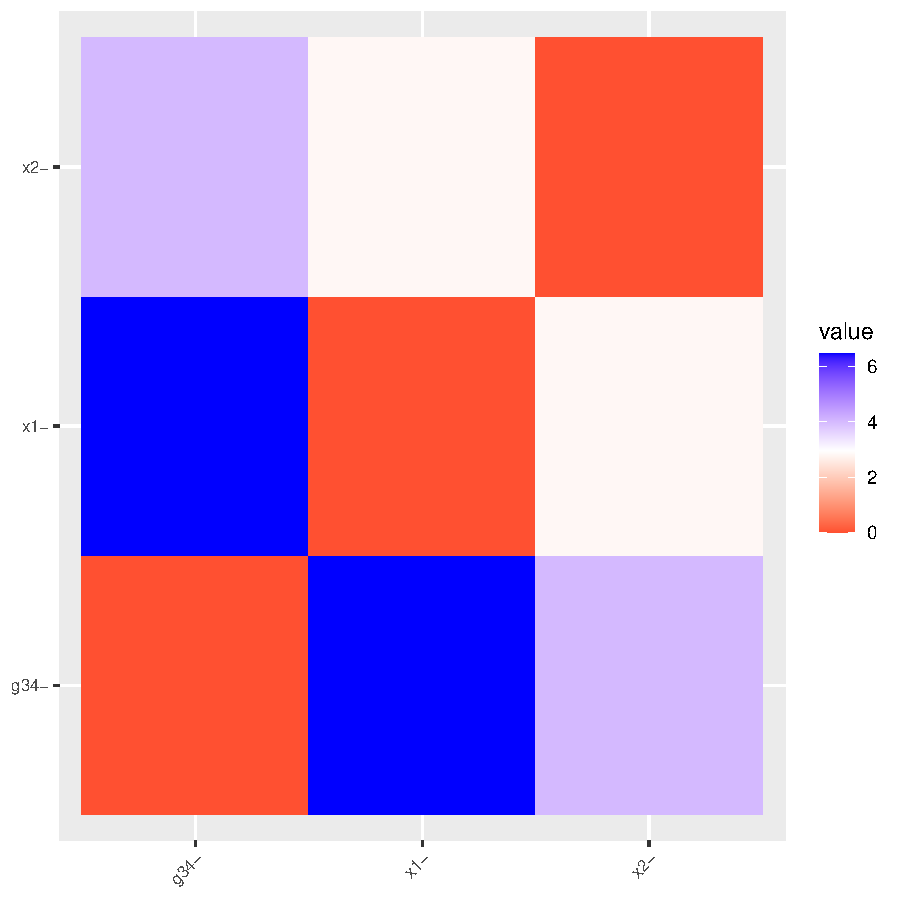
\includegraphics{TP3_M1MAS-002}
Les 2 individus les plus proches sont $x_1$ et $x_2$,est la plus petite, on les regroupe, le centre du groupe composé de ces 2 individus est $g_{12}=(3,11)$ (noeud 6). Le saut de ward correspondant est $(1/2)d(x_1,x_2)=1.41$.
\item Etape final: on regroupe les deux centres 
$g_{12}$ et $g_{34}$.
\begin{Schunk}
\begin{Sinput}
> library("FactoMineR")
> library("factoextra")
> A=matrix(c(2,12,4,10,5,7,4,5),ncol=2, byrow=TRUE)
> X=as.data.frame(A)
> colnames(X)=c("var1", "var2")
> rownames(X)=c("x1", "x2", "x3","x4")
> # Distance euclidienne
> ## CAH sur des données brutes avec hclust ou eclust
> # Distance euclidienne
> dist <- dist(X, method = "euclidean")
> # CAH avec Ward (option ward.D2 avec les distances au carré ou ward)
> hc <- hclust(dist, method = "ward.D2")
> # Figure
> plot(hc, cex = 0.5)
> ##CAH avec eclust de factoextra
> hc2 <- eclust(X, k.max=3,"hclust")
> # dendrogamme
> fviz_dend(hc2) 
> ## Couper le dendogramme pour avoir 2 classes
> coupe <- hcut(X, k = 2, hc_method = "complete")
> # Visualiser le dendrogramme avec les 2 classes
> fviz_dend(coupe, show_labels = FALSE, rect = TRUE)
> # Visualiser les classes en fonction des variables
> fviz_cluster(coupe, ellipse.type = "convex")
> # Visualize silhouhette information
> fviz_silhouette(coupe)
\end{Sinput}
\begin{Soutput}
  cluster size ave.sil.width
1       1    2          0.44
2       2    2          0.57
\end{Soutput}
\end{Schunk}
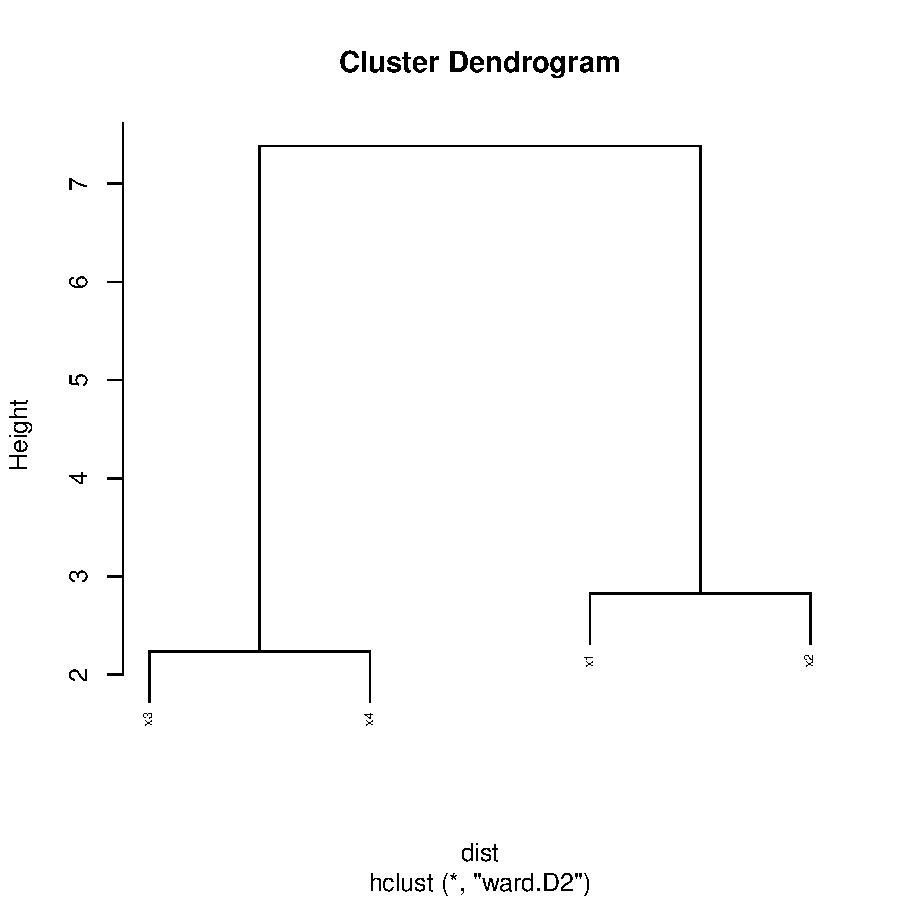
\includegraphics{TP3_M1MAS-003}
\end{itemize}



\item K-means avec $K=2$ classes et des graines initiales $x_1$ et $x_3$.

\begin{itemize}
\item Etape 1:  $x_2$ est plus proche de  $x_1$ que de  $x_3$, on l'affecte alors au groupe de  $x_1$;  $x_4$ est plus proche de  $x_3$ que la graien  $x_1$, on l'affecte alors au groupe de  $x_3$. On a alors les groupes $C_1^1=\{x_1,x_2\}$ et  $C_2^1=\{x_3,x_4\}$
\item On calcule les distances entre les centres $g_1=(3,11)$ et $g_2=(4.5,6)$  des groupes $C_1$ et $C_2$ et les individus: 
\begin{Schunk}
\begin{Sinput}
> library("FactoMineR")
> library("factoextra")
> A=matrix(c(2,12,4,10,5,7,4,5,3,11,4.5,6),ncol=2, byrow=TRUE)
> X=as.data.frame(A)
> colnames(X)=c("var1", "var2")
> rownames(X)=c("x1", "x2", "x3", "x4", "g1", "g2")
> # Distance euclidienne
> dist <- dist(X, method = "euclidean")
> dist
\end{Sinput}
\begin{Soutput}
         x1       x2       x3       x4       g1
x2 2.828427                                    
x3 5.830952 3.162278                           
x4 7.280110 5.000000 2.236068                  
g1 1.414214 1.414214 4.472136 6.082763         
g2 6.500000 4.031129 1.118034 1.118034 5.220153
\end{Soutput}
\end{Schunk}
On remarque que $d(x_1,g_1)<d(x_1,g_2)$ et $d(x_2,g_1)<d(x_2,g_2)$ et $d(x_3,g_2)<d(x_3,g_1)$ et $d(x_4,g_2)<d(x_4,g_1)$ donc les deux groupes ne changent pas: $C_1^2=C_1^1=\{x_1,x_2\}$ et  $C_2^2=C_2^1=\{x_3,x_4\}$. 
\item Etape final: la partition en 2 classes est 
$C_1=\{x_1,x_2\}$ et  $C_2=\{x_3,x_4\}$

\begin{Schunk}
\begin{Sinput}
> A=matrix(c(2,12,4,10,5,7,4,5),ncol=2, byrow=TRUE)
> X=as.data.frame(A)
> colnames(X)=c("var1", "var2")
> rownames(X)=c("x1", "x2", "x3", "x4")
> ##K-means
> km <- eclust(X, "kmeans", k=2)
> km$cluster
\end{Sinput}
\begin{Soutput}
x1 x2 x3 x4 
 1  1  2  2 
\end{Soutput}
\begin{Sinput}
> # Visualisation
> fviz_cluster(km, geom = "text")
> ## Choix de k
> km <- eclust(X, "kmeans", nstart = 2, k.max=3)
> ##Gap
> fviz_gap_stat(km$gap_stat)
> 
\end{Sinput}
\end{Schunk}
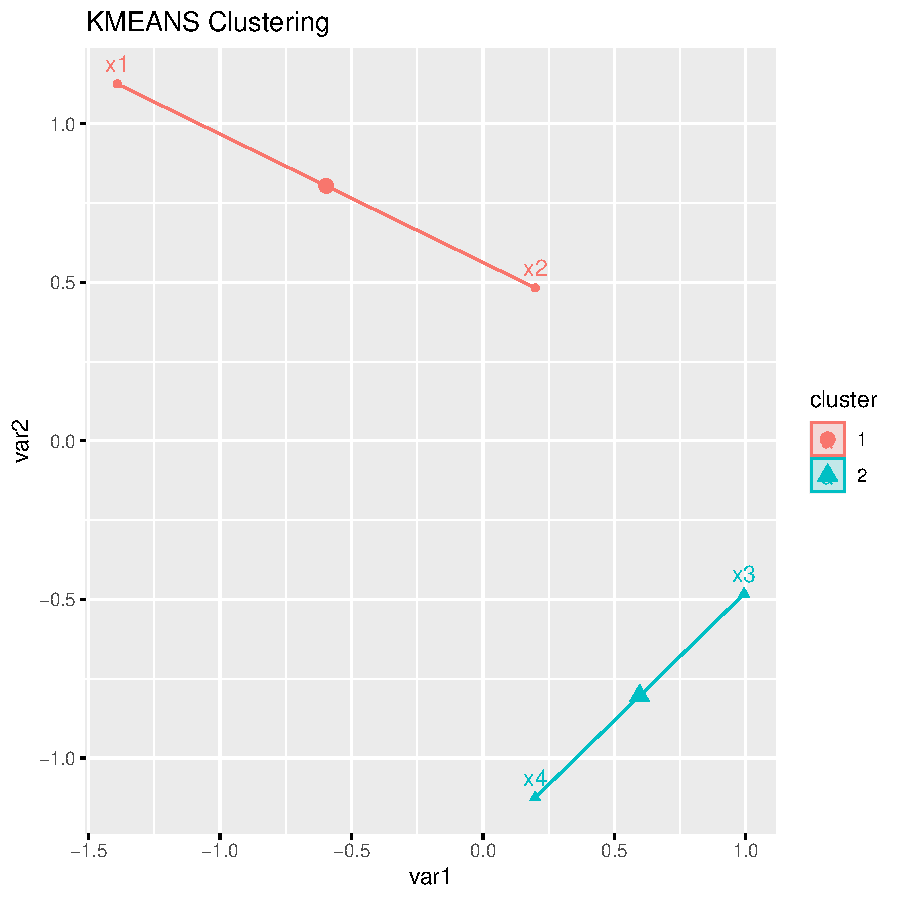
\includegraphics{TP3_M1MAS-005}
\end{itemize}



\end{itemize}


\section{Exemple 2} 
\begin{Schunk}
\begin{Sinput}
> boeufs=read.table("/Users/Sandro/Documents/R/AD/data_boeufs.txt",header=TRUE,dec=',')
> library("FactoMineR")
> library("factoextra")
> activedata=boeufs[,2:7]
> pca <- PCA(activedata, graph = FALSE)
> # CAH sur les résultats de l'ACP
> res <- HCPC(pca, graph = FALSE)
> ## Dendogramme suggére 3 classes
> fviz_dend(res, cex = 0.7, palette = "jco", rect = TRUE, rect_fill = TRUE, # ajouter des rectangles autour des groupes 
+ rect_border = "jco"          # bordures rectangle 
+ )
> ## Les classes sur les plans factoriels
> fviz_cluster(res,repel = TRUE, show.clust.cent = TRUE, # montrer les  centres des classes
+ palette = "jco",ggtheme = theme_minimal(),main = "Factor map"
+ )
> ## Données avec classes
> head(res$data.clust, 10)
\end{Sinput}
\begin{Soutput}
   P_VIF P_CAR P_QUALI P_TOTAL P_GRAS P_OS clust
1    395   224    35.1    79.1    6.0 14.9     3
2    410   232    31.9    73.4    9.7 16.4     2
3    405   233    30.7    76.5    7.5 16.5     2
4    405   240    30.4    75.3    8.7 16.0     2
5    390   217    31.9    76.5    7.8 15.7     3
6    405   243    32.1    77.4    7.1 15.5     2
7    390   229    32.1    78.4    4.6 17.0     3
8    405   240    31.1    76.5    8.2 15.3     2
9    420   234    32.4    76.0    7.2 16.8     2
10   390   223    33.8    77.0    6.2 16.8     3
\end{Soutput}
\begin{Sinput}
> ## Variables qui décrivent le plus les classes
> res$desc.var$quanti
\end{Sinput}
\begin{Soutput}
$`1`
           v.test Mean in category Overall mean sd in category Overall sd
P_GRAS   3.568467         10.84545     8.973913       1.676774   2.355238
P_CAR   -2.414696        224.27273   228.826087       5.738085   8.468110
P_TOTAL -3.901384         72.56364    74.669565       1.236765   2.424052
P_QUALI -4.032590         27.66364    29.921739       1.280818   2.514645
             p.value
P_GRAS  3.590754e-04
P_CAR   1.574833e-02
P_TOTAL 9.564413e-05
P_QUALI 5.516553e-05

$`2`
        v.test Mean in category Overall mean sd in category Overall sd
P_CAR 3.518013         238.4286     228.8261       5.205962   8.468110
P_VIF 3.350894         409.2857     401.1739       5.624291   7.510295
           p.value
P_CAR 0.0004347903
P_VIF 0.0008055122

$`3`
           v.test Mean in category Overall mean sd in category Overall sd
P_TOTAL  3.110855            77.72    74.669565      0.9368031   2.424052
P_QUALI  2.947493            32.92    29.921739      1.3212116   2.514645
P_VIF   -2.690501           393.00   401.173913      4.0000000   7.510295
P_GRAS  -3.058454             6.06     8.973913      1.0307279   2.355238
            p.value
P_TOTAL 0.001865463
P_QUALI 0.003203620
P_VIF   0.007134492
P_GRAS  0.002224825
\end{Soutput}
\begin{Sinput}
> ## Les composantes qui sont le plus associées aux classes
> res$desc.axes$quanti
\end{Sinput}
\begin{Soutput}
$`1`
         v.test Mean in category Overall mean sd in category Overall sd
Dim.1 -4.094274        -1.566105 3.240162e-15      0.9297269   1.717754
           p.value
Dim.1 4.234935e-05

$`2`
       v.test Mean in category Overall mean sd in category Overall sd
Dim.2 3.48012         1.430149 1.466043e-14      0.6285289   1.274933
           p.value
Dim.2 0.0005011886

$`3`
         v.test Mean in category Overall mean sd in category Overall sd
Dim.1  2.804409         1.948688 3.240162e-15      0.6620154   1.717754
Dim.2 -2.797100        -1.442565 1.466043e-14      0.5509465   1.274933
          p.value
Dim.1 0.005040893
Dim.2 0.005156353
\end{Soutput}
\begin{Sinput}
> ## Les individus qui représent le plus les classes
> res$desc.ind$para
\end{Sinput}
\begin{Soutput}
Cluster: 1
      13       17       16       21       22 
1.045618 1.347510 1.425291 1.509209 1.538045 
------------------------------------------------------------ 
Cluster: 2
        4         8         3         6        11 
0.7789460 0.9785818 1.0420378 1.2698386 1.3023214 
------------------------------------------------------------ 
Cluster: 3
       10         7         5         1        12 
0.6910894 0.9927218 1.6723445 1.8951912 2.3630145 
\end{Soutput}
\begin{Sinput}
> ## Interface graphique
> 
> #require(Factoshiny)
> #hc4 <- HCPCshiny(activedata)
> 
> ## K-means avec 3 classes
> 
> km <- eclust(activedata, "kmeans", k=3)
> ## Choix de k
> km <- eclust(activedata, "kmeans", nstart = 2, k.max=10)
> km
\end{Sinput}
\begin{Soutput}
K-means clustering with 1 clusters of sizes 23

Cluster means:
     P_VIF    P_CAR  P_QUALI  P_TOTAL   P_GRAS     P_OS
1 401.1739 228.8261 29.92174 74.66957 8.973913 16.42174

Clustering vector:
 [1] 1 1 1 1 1 1 1 1 1 1 1 1 1 1 1 1 1 1 1 1 1 1 1

Within cluster sum of squares by cluster:
[1] 3382.92
 (between_SS / total_SS =  -0.0 %)

Available components:

 [1] "cluster"      "centers"      "totss"        "withinss"     "tot.withinss"
 [6] "betweenss"    "size"         "iter"         "ifault"       "clust_plot"  
[11] "nbclust"      "data"         "gap_stat"    
\end{Soutput}
\begin{Sinput}
> fviz_gap_stat(km$gap_stat)
\end{Sinput}
\end{Schunk}
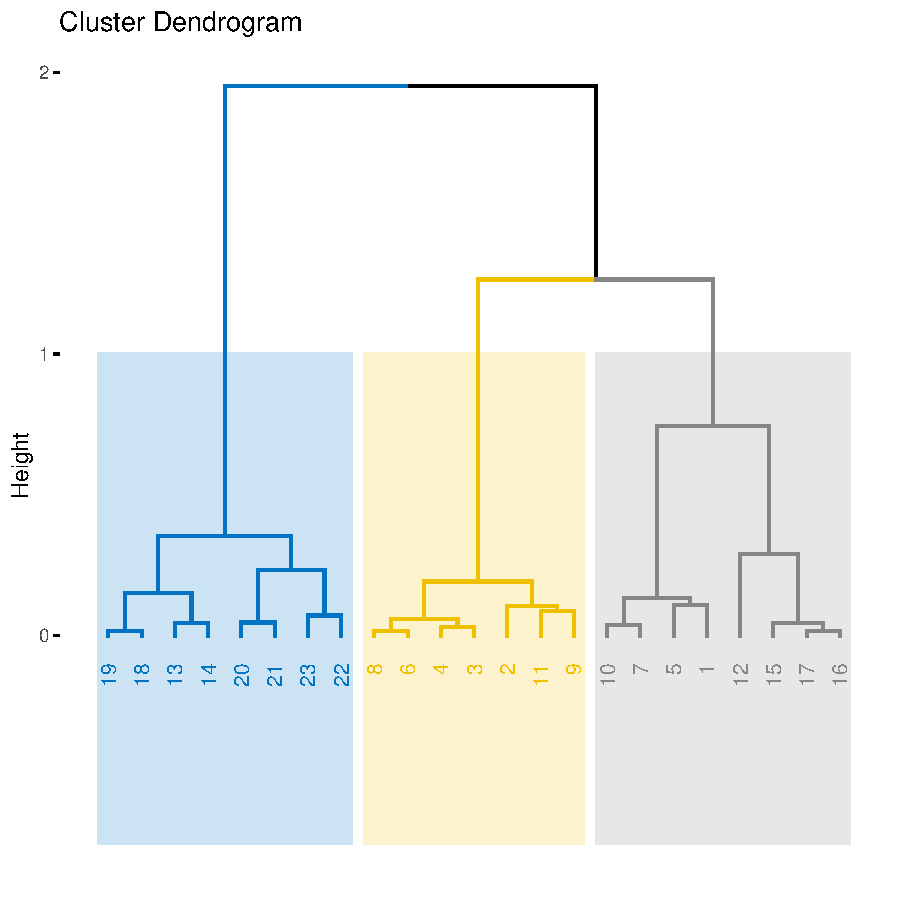
\includegraphics{TP3_M1MAS-006}

\end{document}
